\section{Arithmetic}
The arithmetic construct was the first thing implemented.
It is a standalone piece of code only exposing a single method, Parse, which takes a string representing an equation and returning a tuple of the evaluated value and an error.
Because of this isolation I created it as a subpackage which also allowed me to simplify the error handling.

I was able to panic and recover\footnote{Panic is similar to an exception in other languages but has different semantics. Errors in Go should be passed through the use of multiple return values instead.} to completely unwind the parser and lexer.
Although panics are reserved for truly exceptional cases in Go, they had to be used in this case.
Errors encountered during lexing or parsing of a language are almost always fatal as they leave the system in an indeterminate state.
For example, the following make no sense in the context of a POSIX shell equation:
\begin{verbatim}
++
  or
35 67 89
\end{verbatim}
This is an implementation detail and can of course be treated differently.
In bash the '++' symbol can represent post-increment or pre-increment depending on its position.
The numbers could also be joined together into a single literal; Python and Java do something similar with underscores rather than spaces\cite{UNDERSCORE-NUM-LITERAL}.

One of Go's golden rules is 'never raise a panic across package boundaries' and to do this we defer\footnote{A Go construct that allows running a final function no matter how the function returns. the os.Exit is the only way to skip these.} a recover function.
If recover detects we have panicked it checks to see if it was a panic we created.
If it was then it is turned into an error and retuned normally. 
Runtime errors are allowed to crash the program.

During testing it was discovered that in the case of zero division the checks where not through enough the was allowed panic to bubble up rather than being converted into an informative error. 
The fix for this would be the addition of a division helper function similar to that used for shifting (See \ref{lst:arith-shift}) which would catch the runtime panic and raise a custom one that could be detected properly. XXX % Add reference to integration test that caught it.

\newpage %XXX NEWPAGE 
\subsection{Lexer}
The Lexer was completed during the first iteration as planned and has a good set of unit tests that where used to ensure the correctness of returned tokens.

The syntax for equations can consist of just variable names, symbols and numeric literals.

Variable names are detected using a state machine version of the following regular expression, \verb![a-zA-Z_][a-zA-Z0-9_]*!.

POSIX requires that detection of numeric values can be done in base 8 (Octal), 10 (Decimal) and 16 (Hexadecimal).
Values are always converted to base 10 for use inside the lexer.
If the literal is invalid, e.g \verb!0xffk! an error is returned that unwinds the parser.
The Scope struct (See~\ref{sec:scope}) does not yet have a way to perform transactions so any assignments that have already been conducted when an error occurs will persist.
Figure~\ref{fig:arith-assign-fail} shows that dash also does this and the spec does not mention how it should work.

\begin{figure}[hp]
    \centering
    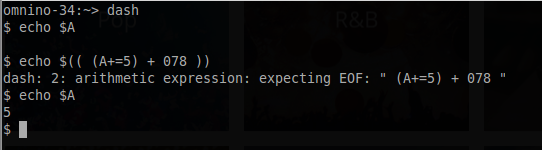
\includegraphics[width=0.8\textwidth]{arith-fail-with-assign.png}
    \caption[Dash assignment even with an error]{The text shown when the error occurs is very uninformative. bash does a slightly better job but still assigns to the variable.}
    \label{fig:arith-assign-fail}
\end{figure}

Symbols are the simplest thing to detect (See code in~\ref{lst:arith-symbol-lex}).
They only require one character of lookahead to be determined from any other symbol.
Some symbols also have an assignment variant.
If we encounter a symbol where this is possible, e.g '+',  a flag it set that will cause a check for a subsequent equal symbol.
If one is found the code takes advantage of the definition order of the tokens to change them to their equivalents.

\subsection{Parser}
The parser was not completed along with the lexer in the first iteration as had been planned.
It was finished in the second one along with extensions to Scope.

The tokens passed from the lexer are assigned to their node type by a simple switch statement.
These node types are used to abstract the functionality of similar operations.
For example $a + b$, $a * b$ and $a \mathrel{+}= b$, $a \mathrel{*}= b$ show that behaviour is similar and it is just the operation that differs in most cases .
Respectively they would be created as Infix and InfixAssign nodes with a value set to indicate what operation is desired.
Operations are functions that are stored in a hash tables for each type of node.

The Pratt parser requires that each node have two functions and one value, see~\ref{lst:arith-node-interface}.
Since Go interfaces can only consist of methods I just changed the value to a getter method instead.

\subsection{Variables}
To begin with I created stub methods on the parser that would eventually interact with the supplied scope.
When arithmetic was complete and I started work on the Scope these methods where changed to actually work.

Values are converted to strings before being stored.
If a retrieved variable can be parsed as octal, decimal or hex they are converted to base 10 before being returned and used.
If a variable cannot be parsed as a number or doesn't exist a value of zero is used instead.

Variables can only be accessed by using their unprefixed form, i.e \verb!(( a = 5 ))! will work, but \verb!(( $a = 5 ))! will not.
This is because variable expansion is a separate process and is done before arithmetic expansion.
Because of the flawed lexer design prefixed variables are not detected properly when used inside the construct and will cause an error (See~\ref{sec:main-lexer-arith}).

\subsection{Ternary}
The ternary operator is unique in that it operates on three values.

Unfortunately due to the fact that the tree is evaluated as it is constructed by my version of the pratt parser a bug surfaced.
When both sides of the environment contained assignment operators variables could be modified twice or always assigned the second value.
E.g With \verb!y = 0! an equation like \\ \verb!x ? y += 1 : y += 3! would make \verb!y == 4! no matter which side was meant to execute.

I left the bug with a failing test case while I continued the project.
I then went back to fix it in the last iteration using the knowledge I had gained during the project.

My fix \textit{feels} ugly and I am not completely happy with it despite the fact it works.
Assignments are blocked by setting a flag and then at each significant point of the ternary the position of the lexer is recorded.
When the end of the equation has been detected we record it and rewind the lexer.
The parser runs again across the section of the ternary the condition indicated should be run with the assignment blocking flag turned off.
The lexer is then moved forward to just after the end of the ternary.
This is of course not an ideal solution as three equations are parsed when only one is applied.












